\appendix

\section{Laplace Tidal Equations in Spherical Coordinates \label{app:coords}}

To convert the Laplace Tidal Equations to a spherical coordinate system we must make use of the following well-known identities for the gradient and divergence operators,
\begin{equation}
\nabla f = \frac{1}{R} \partial_{\lambda} f \bm{\hat{\lambda}}  
+ \frac{1}{R \cos{\lambda}} \partial_{\lambda} f \bm{\hat{\phi}}
\end{equation}
\begin{equation}
\nabla \cdot \bm{A} = -\frac{1}{R \cos{\lambda}} \partial_{\lambda} \left( \cos{\lambda}\, A_{\lambda} \right) + \frac{1}{R \cos{\lambda}} \partial_{\phi} A_{\phi}
\end{equation}

where $\bm{A}$ is some vector quantity tangent to the spherical surface, $f$ is a scalar quantity, and $\bm{\hat{\lambda}}$ and $\bm{\hat{\phi}}$ are the latitude and longitude unit vectors, also tangent to the surface. Note that we ignore any component of the divergence and gradient operators in the radial direction in accordance with the shallow water assumptions.

Defining $\bm{u} = \left(u, v \right) = (u_{\phi}, -u_{\lambda} ) $ and using the fact that $\bm{\Omega} = \Omega \bm{\hat{k}}$, where $\bm{\hat{k}}$ is the Cartesian unit vector aligned with the rotation axis, then the continuity equation can be rewritten as,
\begin{equation}
\partial_t \eta + \frac{h_0}{R \cos{\lambda}} \left( \partial_{\lambda}
\left(v \cos{\lambda} \right) +  \partial_{\phi} u \right) = 0 \, .
\end{equation}

\noindent Similarly, the momentum equation becomes, 
\begin{equation}
\partial_t u - 2 \Omega v \sin{\lambda}
+ \alpha u
+\frac{c_D}{h_0} \left(u^2 + v^2 \right)^{\nicefrac{1}{2}} u
+ \frac{g}{R \cos{\lambda}} \partial_{\phi} \eta
= 
(1 + k_2 - h_2) \frac{1}{R \cos{\lambda}} \partial_{\phi} U_2
\end{equation}
\begin{equation}
\partial_t v + 2 \Omega u \sin{\lambda}
+ \alpha v
+\frac{c_D}{h_0} \left(u^2 + v^2 \right)^{\nicefrac{1}{2}} v
+ \frac{g}{R} \partial_{\lambda} \eta
= 
(1 + k_2 - h_2) \frac{1}{R} \partial_{\lambda} U_2
\end{equation}

%
%\section{Finite Difference Energy Expressions \}
%
%For a system experiencing both Rayleigh and bottom friction, the full dissipated energy over an orbit is given by,
%\begin{equation}
%F = \frac{\rho}{4 \pi T} \iint \left[h \alpha \left(u^2 + v^2 \right) + c_D \left(u^2 + v^2 \right)^\nicefrac{3}{2} \right}d\Omega dt,
%\end{equation}
%
%\noindent where $\Omega$ is the solid angle and we assume that $h \ll R$.


\section{Numerical Error and Testing \label{app:error_tests}}

This appendix outlines how numerical error was quantified in this study, as well as several numerical tests that were performed to benchmark our code.

Numerical error is quantified in two distinct ways in this manuscript. Local error, such as that plotted in Figure \ref{fig:spatial_error}, is simply calculated as the percentage error:
\begin{equation}
E_i = \dfrac{\left| x_{i, num} - x_{i, anlyt} \right| }{x_{anlyt}} \times 100 \, .
\end{equation}

To investigate global error at a particular simulation time, such as that shown in figures \ref{fig:temporal_error} and \ref{fig:spatial_convergence}, we use the normalised $L_1$, $L_2$, and $L_{\infty}$ error norms:
\begin{align}
L_1 &= \dfrac{1}{N}\sum_1^N \left| x_{i, num} - x_{i, anlyt} \right| \, , \\
L_2 &= \left( \dfrac{1}{N}\sum_1^N \left| x_{i, num} - x_{i, anlyt} \right|^2 \right)^{\nicefrac{1}{2}}\, , \\
L_{\infty} &= \text{max} \left| x_{i, num} - x_{i, anlyt} \right|\, ,
\end{align}

\noindent where $N$ is the total number of grid points in the model domain, and $i$ is the index of each cell. The normalised approach is common in CFD problems as it allows one to estimate the convergence order of the implemented numerical method.

As with any numerical solution there are errors associated with discretisation of the problem into the model domain. We performed resolution testing across various ocean thicknesses to determine how these errors scale with grid resolution using the semi-analytical solutions of \citet{matsuyama2014tidal} as our benchmark. Although the solutions from \citet{matsuyama2014tidal} are not purely analytical, we use solutions that are truncated at spherical harmonic degree $l=30$. As such, these can be considered the exact solutions. Four of these tests are shown in this section to illustrate that the numerical method and code perform as expected, both as a function of space and time. Tests \numrange{1}{3} were run for Enceladus' eccentricity tide, using $h_0 = \SI{500}{\metre}$, $\alpha = \SI{e-5}{\per\second}$, and $\Delta t = \SI{2}{\second}$. Test 4 was for the obliquity tide on Titan using $h_0 = \SI{1}{\kilo\metre}$ and $\alpha = \SI{e-8}{\per\second}$. The grid was spaced at \SI{1}{\degree} throughout, except in tests 3 and 4 which examine how the numerical error depends on model resolution.

\begin{figure}
\centering
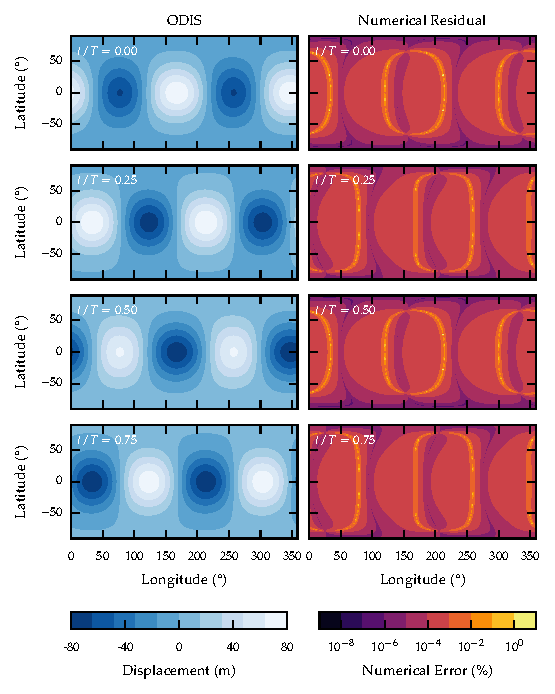
\includegraphics[width=0.85\linewidth]{Figures/spatial_error_ecc}
\caption{Displacement solutions (left column) and corresponding percentage error (right column) for Enceladus' eccentricity tide with $h_0 = \SI{500}{\metre}$ and $\alpha = \SI{e-5}{\per\second}$. The numerical grid was spaced at \SI{1}{\degree}. Each row corresponds to a different time interval throughout one orbital period, $T$. Percentage eror is  $< \SI{0.01}{\percent}$ over much of the model domain, with local highs where the solution passes from postive to negative displacement. \label{fig:spatial_error}}
\end{figure}


\begin{figure}[t]
\centering
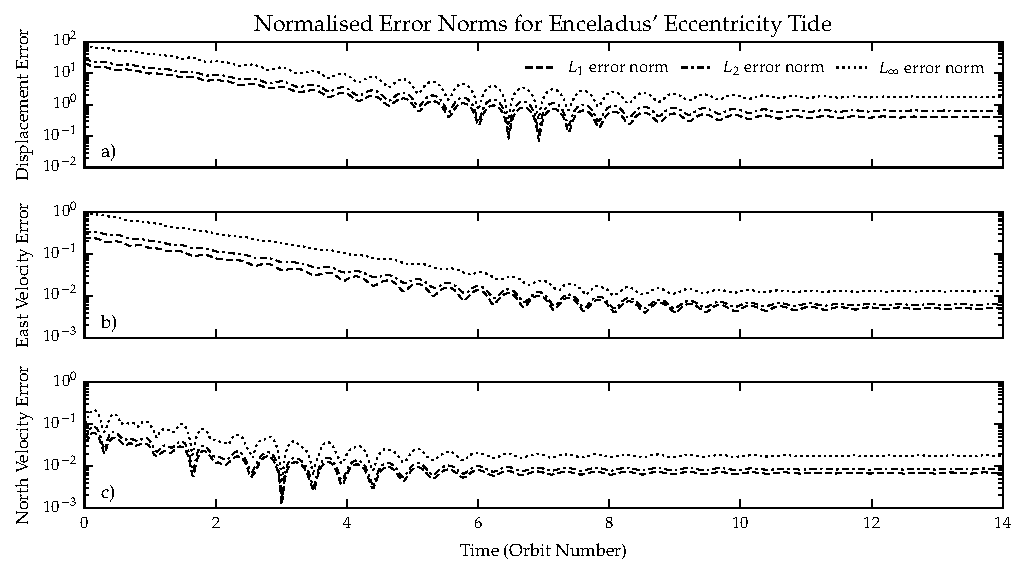
\includegraphics[width=\linewidth]{Figures/temporal_error_ecc}
\caption{Normalised error norms as a function of time for Enceladus' eccentricity tide with $h_0 = \SI{500}{\metre}$ and $\alpha = \SI{e-5}{\per\second}$. At approximately \num{10} orbits, all parts of the solution have converged after which the normalised error remains small, and oscillates over the orbital period. \label{fig:temporal_error}}
\end{figure}


\begin{figure}[t]
\centering
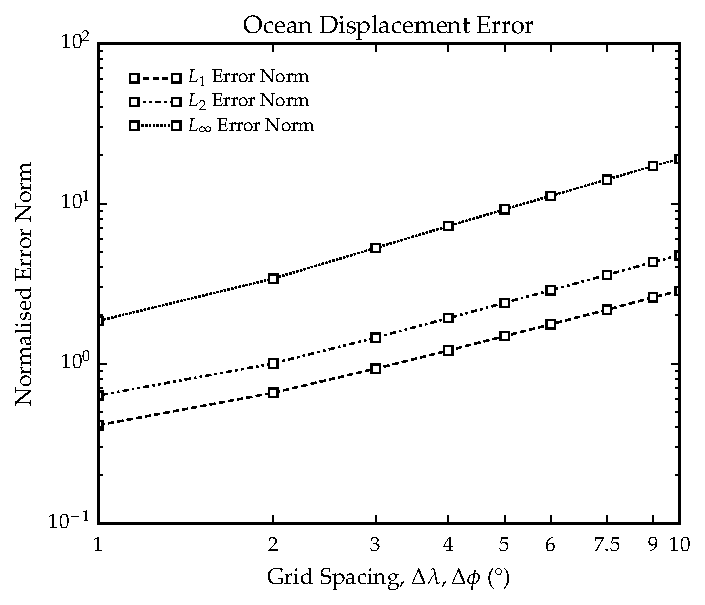
\includegraphics[width=0.6\linewidth]{Figures/convergence_eta}
\caption{Normalised error norms as a function of time for Enceladus' eccentricity tide with $h_0 = \SI{500}{\metre}$ and $\alpha = \SI{e-5}{\per\second}$, taken at pericenter at the beginning of orbit \num{100}. A least-squares fit to each error norm in log-log space yields slopes of \num{0.86}, \num{0.90} and \num{1.03} for the $L_1$, $L_2$ and $L_{\infty}$ normalised error norms, respectively. \label{fig:spatial_convergence}}
\end{figure}



\begin{figure*}[!t]
    \centering
    \begin{subfigure}[t]{\linewidth} % contains the two plots in a single figure
        \includegraphics[width=\linewidth]{Figures/convergence_dissipation}
        \phantomcaption
        \label{fig:conv_a}
    \end{subfigure}
    \begin{subfigure}[t]{0\linewidth} % the hidden unwanted image
         \includegraphics[width=\linewidth]{Figures/convergence_dissipation}
         \phantomcaption
         \label{fig:conv_b}   
    \end{subfigure}
    \vspace{-0.5cm}
\caption{Dissipation convergence and error scaling as a function of grid resolution. Panel \ref{fig:conv_a} shows the time evolution of the orbit-averaged dissipated energy at periapsis. The solid lines represents different grid resolutions, whereas the dashed line is the semi-analytical solution for Rayleigh drag from \citet{matsuyama2014tidal}. Panel \ref{fig:conv_b} shows the dissipation error between the numerical and semi-analytical solutions with increasing resolution. The least-squares slope of the first six data points (when the slope is steady) in log-log space is \num{1.94}. These simulations are for the obliquity tide using $h_0 = \SI{1}{\kilo\metre}$ and $\alpha = \SI{e-8}{\per\second}$ on Titan. \label{fig:conv}}
\end{figure*}

It is important to understand how the model resolves the solution across the numerical domain, especially when using the fixed latitude-longitude grid employed here. This is done in test 1 (Figure \ref{fig:spatial_error}) where the ocean surface displacement (left) is compared to the corresponding error field (right). The ocean configuration is near a gravity-wave resonance, so it is easy to discern the eastward propagating gravity-wave through the model domain at each time slice. Percentage error in the numerical model is very small ($< \SI{0.01}{\percent}$) over the majority of the domain. Near the poles, where grid points are closely arranged, numerical error is smallest. At the zero-crossing in displacement both the numerical and semi-analytical solutions become $\ll \SI{1}{\metre}$. As a result, the numerical error locally spikes in those regions producing the rings of increased error seen in Figure \ref{fig:spatial_error}. Overall, the numerical error is very low, giving us confidence in the ability of ODIS to spatially resolve the solutions.

As the tidal forcing in this problem is periodic, one expects the solution and its corresponding error to also be periodic. It is therefore logical to investigate how the numerical error changes over time. We investigate this in our second test, starting the numerical simulations from an undisturbed and unforced ocean. This is shown in Figure \ref{fig:temporal_error}, where once again the numerical error is computed against the \citet{matsuyama2014tidal} semi-analytical solutions. The error is quantified using the normalised $L_1$, $L_2$ and $L_{\infty}$ error norms, defined above. The maximum error in each solution is given by the $L_{\infty}$ norm. Normalised error is greatest at the beginning of the simulation, as this is during the model ``spin-up'' time. After approximately \num{10} orbits both the displacement and two velocity solutions converge. At this point the average error over each orbital period remains constant. The magnitude of this converged error is a function of the grid resolution, as shown in test 3. Once converged, the normalised error oscillates over the orbital period. This is expected; the maximum gradients in all three solutions periodically vary over an orbit. In regions where these gradients are maximised the finite difference scheme produces the poorest approximation. Consequently, the error varies as a function of time, even after convergence. 

\textbf{As with most numerical methods, the inherent error associated with discretization builds up over time. Figure B.12 shows the error from a short simulation. Only when running the same simulation for several years of simulation time does the numerical error become great enough to show an appreciable departure from the analytical solution. This becomes more significant with small drag coefficients, when the solution is the least dampened. For the bodies studied in this paper, numerical convergence is reached well before numerical error becomes significant.}

In order to verify if the numerical scheme is implemented properly, it is prudent to perform convergence analysis on the numerical solutions. Figure \ref{fig:spatial_convergence} shows this analysis in our third test. The normalised error norms are plotted with varying grid resolution, spanning \SIrange{1}{10}{\degree} in both longitude and latitude. As expected, the accuracy of the numerical solution increases with decreasing grid size. With increasing resolution the local approximation of spatial derivatives improves, which is what produces this general trend. The rate at which the errors are reduced as a function of resolution is known as the order of convergence. This can be estimated by finding the slope of the normalised error norms in log-log space. Using a least-squares fit we find slopes of \num{0.86}, \num{0.90} and \num{1.03} for the $L_1$, $L_2$ and $L_{\infty}$ normalised error norms, respectively. We therefore conclude that the order of convergence of the numerical method implemented in ODIS is $\sim 1$, which is expected for the finite difference expansions made in equations \ref{eq:gen1} and \ref{eq:gen2}.

The total dissipated energy is of fundamental importance from the point of view of the Planetary Science community. As our final test we therefore investigate how the numerical dissipation solution varies as a function of time and grid resolution, shown in Figure \ref{fig:conv}. Unlike the other tests, this is run for the obliquity tide on Titan with an ocean of $h_0 = \SI{1}{\kilo\metre}$ and $\alpha = \SI{e-8}{\per\second}$. The numerical time- and orbit-averaged dissipated energy oscillates over time until converging to a single value, shown in the left panel. This final value gradually approaches the \citet{matsuyama2014tidal} semi-analytical solution as grid resolution is increased. The right panel, similar to Figure \ref{fig:spatial_convergence}, plots the numerical percentage error as a function of grid spacing. Again, the error decreases with decreasing grid spacing. The order of convergence for the dissipation is once again given by the slope of the line in Figure \ref{fig:conv_b}, which approaches $\sim 2$.

Based on these resolution tests, all simulations were ran for grid resolutions of \SIrange{1}{3}{\degree} in latitude and longitude.